\chapter{Introduction}\label{chapter:introduction}

Functional lists (\autoref{fig:example-list}) are a handy and easy-to-use data structure in functional programming. However, compared to imperative arrays, |lookup| and |update| operations on lists have a significantly worse runtime of $\mathcal{O}(n)$ instead of $\mathcal{O}(1)$. 

\begin{figure}[htpb]
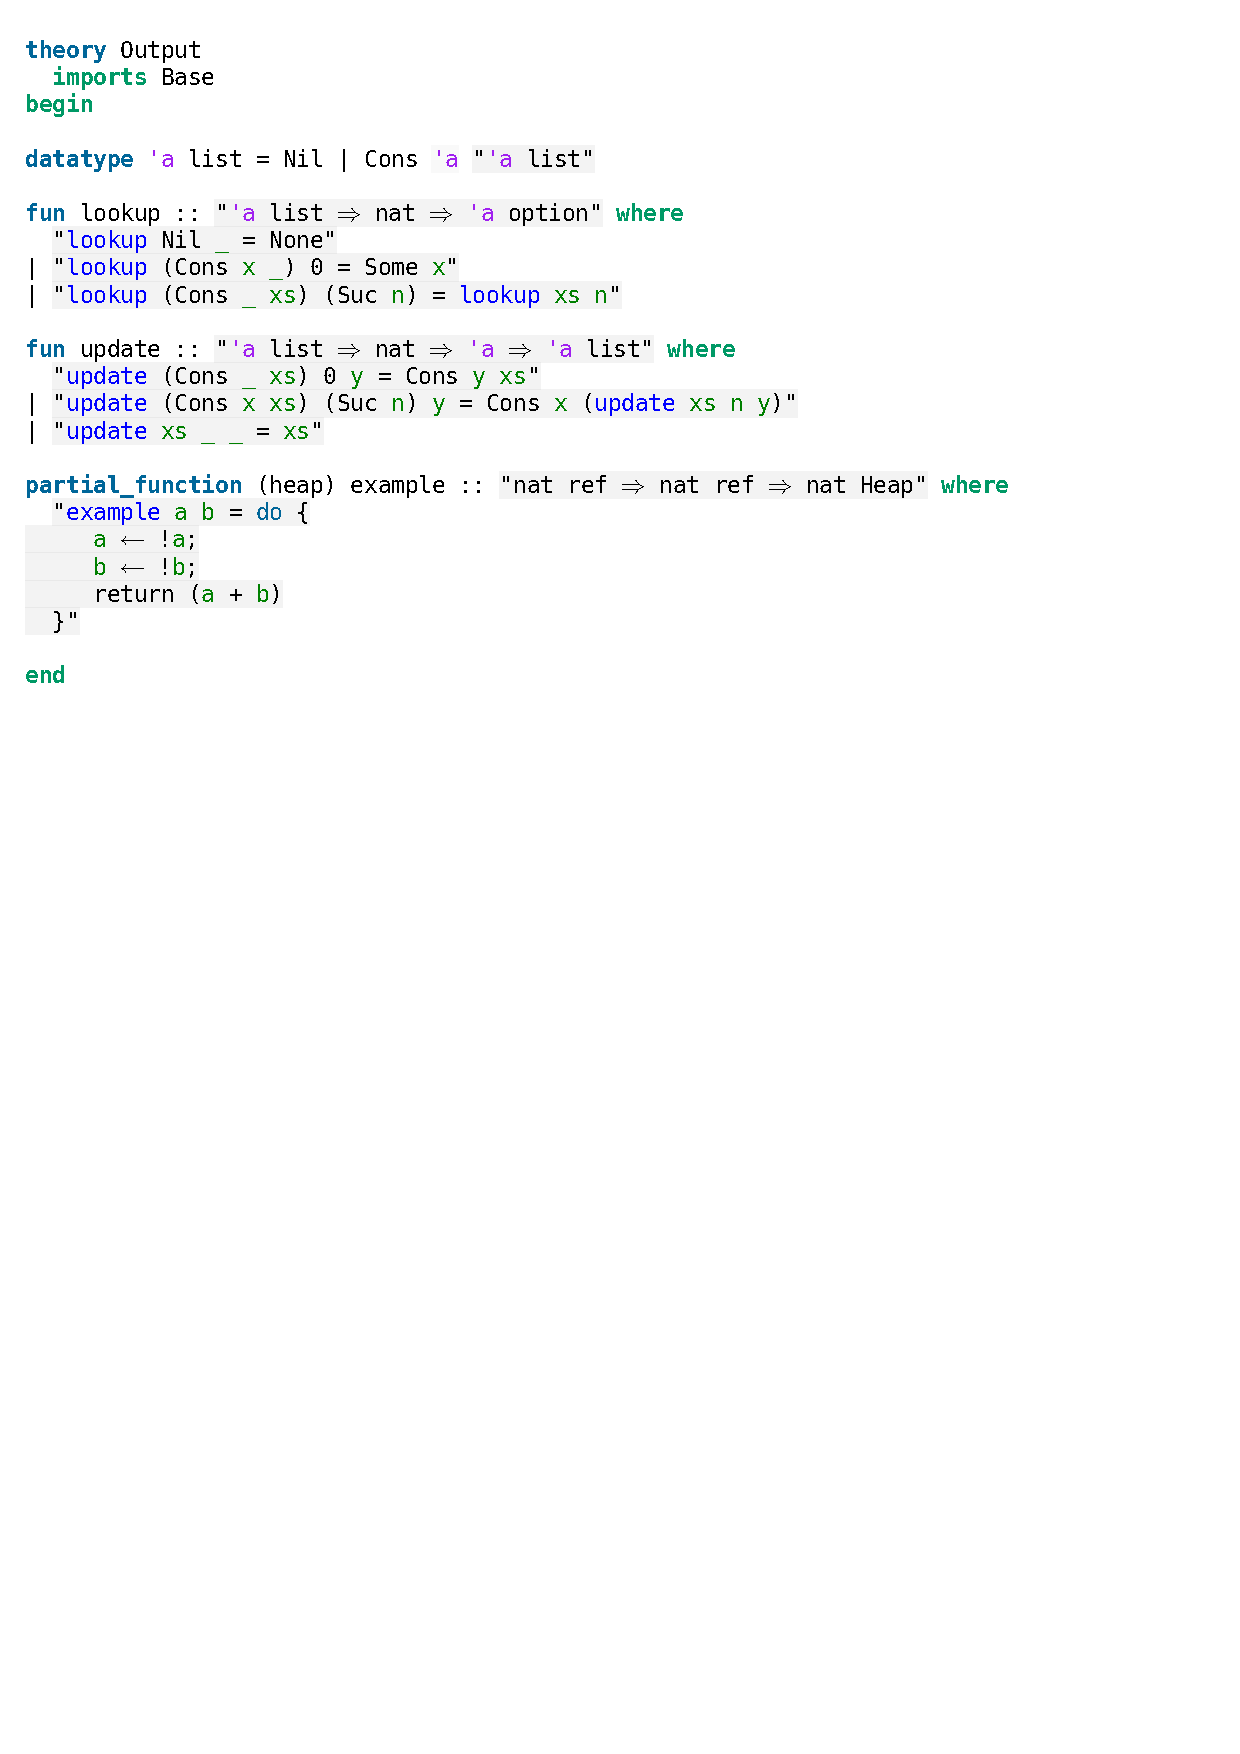
\includegraphics[trim={0 22,2cm 0 2,3cm},clip, width=1.00\textwidth]{figures/Theory_Intro.pdf}
\caption[Example functional list implementation]{An example implementation of a functional list.}\label{fig:example-list}
\end{figure}

\noindent Then why not replace lists with arrays at compile time? Like that, we can preserve the functional language's methodological benefits and the runtime of imperative arrays. In \autoref{section:hnr_arr}, we will apply this simple method. But the problem with the method is that arrays are ephemeral, meaning that updates are destructive, like for most imperative data structures \parencite[p.2]{Okasaki_1998}. Contrary to imperative languages, all data structures are automatically persistent in functional languages \parencite[p.2]{Okasaki_1998}.
If we use a list in a non-linear way, we would need to copy the corresponding array, which is costly in terms of runtime and memory. \\
To cope with that, we use diff arrays (\autoref{chapter:diff-array}), also called trailer arrays \parencite{Bloss1989}, which store their updates in a tree-like structure next to the array \parencite[p.706]{Kumar2017}. 
With them, we can have lookup and update operations in $\mathcal{O}(1)$ for the most recent version of the data structure. \\
This thesis aims to automatically convert functional programs using lists to imperative ones using (diff) arrays. Additionally, we will automatically create equivalence proofs to ensure that the two versions of the program are doing the same. We use the Isabelle/HOL theorem prover (\autoref{chapter:isabelle}) for this purpose. We can reason about imperative programs using Isabelle's Imperative/HOL framework (\autoref{section:imperative_hol}) and a separation logic (\autoref{chapter:separation-logic}) built on top of it. Using this setup, we implemented an infrastructure to parallelly translate the functional programs to imperative ones and create equivalence proofs (\autoref{chapter:automatic-refinement}).
